\begin{figure*}[htbp!]
	\centering
	\includegraphics[width=0.9\linewidth]{imgs/Fig06_WatdivTemplateTypes}
	\caption{Average Runtime per BGP type.}
	\label{fig:Fig06_WatdivTemplateTypes}
\end{figure*}

Only comparing query runtimes might be an oversimplification in benchmark analysis. 
When comparing batch runtimes the slow tail of the distributions dominates the average runtimes. In section~\ref{subsec:templates} we investigate whether certain query templates dominate the batch runtimes.
Query execution times depend on the state of the database, which motivates studying the query context. Previous results are still valid as all queries are executed 5 times and each time the median is taken to calculate batch runtimes.

In section~\ref{subsec:load} we study the effect of the server load on the query runtimes by comparing a single-client benchmark with a stress test with 5 clients. What queries have been executed previously might also affect query runtimes due to result caching. This will be explored in section~\ref{subsec:caching}. Often not reported, but the effect of result completeness can have a big impact on the query runtimes reported, as we will discuss in section~\ref{subsec:completeness}.

\subsection{Query runtimes for different template types}
\label{subsec:templates}

%
%RESULTS Rev1: Notebook Rev1_14

%Bla_N1_64_W1000_Opt Gra_N1_64_W1000_Opt ES_N1_64_W1000_Def Vir_N1_64_W1000_Opt LDF_N1_64_W1000_Def
%template_type 					
%C 	10.953371 	33.118651 	300.000000 	29.163331 	300.0
%F 	0.710602 	1.041088 	112.866074 	0.551893 	300.0
%L 	0.567620 	1.054375 	25.129921 	0.191519 	300.0
%S 	0.634281 	0.427514 	26.836085 	0.083854 	300.0
%
%
%
%Bla_N1_64_W1000_Opt Gra_N1_64_W1000_Opt ES_N1_64_W1000_Def Vir_N1_64_W1000_Opt 	LDF_N1_64_W1000_Def
%template 					
%C1 	4.853528 	41.074082 	300.000000 	50.148527 	300.000000	Bla
%C2 	17.724176 	25.320613 	300.000000 	10.052103 	300.000000	Vir
%F1 	0.651362 	0.590807 	10.350239 	0.064754 	300.000000	Vir
%F2 	0.769873 	1.529352 	133.287122 	4.005216 	300.000000	Bla
%F3 	1.176846 	2.933791 	300.000000 	4.955930 	300.000000	Bla3
%F4 	0.887820 	4.861341 	300.000000 	0.668484 	300.000000	Vir
%F5 	0.064486 	0.060477 	2.468437 	0.019201 	6.090464	Vir
%L1 	0.035158 	0.006558 	1.346970 	0.007135 	2.848204	Vir
%L2 	1.650052 	2.166173 	25.129921 	0.302525 	300.000000	Vir
%L3 	0.037243 	0.009755 	1.025530 	0.006762 	2.260012	Vir
%L4 	0.791782 	4.210585 	51.241839 	0.370861 	300.000000	Vir
%L5 	1.185084 	4.131350 	122.003833 	0.317177 	300.000000	Vir
%S1 	0.046855 	0.011460 	3.790836 	0.137013 	4.298328	Gra
%S2 	0.941007 	2.177947 	46.095154 	0.160746 	300.000000	Vir
%S3 	1.636567 	0.445906 	26.885182 	0.069650 	300.000000 	Vir
%S4 	0.670550 	0.411107 	81.268466 	0.084230 	300.000000	Vir
%S5 	1.026515 	0.458653 	300.000000 	0.070567 	300.000000	Vir
%S6 	0.206022 	0.141913 	7.889212 	3.760982 	300.000000  Gra
%S7 	0.037128 	0.005170 	0.295254 	0.005701 	0.945705	Gra3
%\caption{Average Runtime per query template for 5 single-node setups. \textbf{TPF1\_64} has only 5 templates which do not coincide with the timeout of 300s, for \textbf{ES1\_64\_Def} this is alread 15 templates.
%\textbf{Vir1\_64\_Opt} is the fastest engine for 13 templates, \textbf{Gra1\_64\_Opt} for and \textbf{Bla1\_64\_Opt} for 3 templates each. Template \textbf{C3} was omitted due to query completeness issues. Blazegraph was the only engine to retrieve all results. } 
The queries of the WatDiv benchmarks are all BGPs but have different shapes and selectivity properties. The benchmark generator has 20 templates which can be further organized into 4 template categories (shapes). 
In Figure~\ref{fig:Fig06_WatdivTemplateTypes} we show the average runtime per template for 5 stores on WatDiv1000M.
\begin{itemize}
	\item \textbf{Template timeouts:} For \textbf{TPF1\_64} 15 runtime averages coincide with the benchmark timeout (300s). Successful queries are spread out over the different types: \textbf{F}:1, \textbf{S}:2, \textbf{L}:2.
	\textbf{ES1\_64\_Def} has timeouts for the 2 \textbf{C} queries,  2 \textbf{F} queries, and 1 \textbf{S} query. The other stores have no averages close to timeout.
	
	\item  \textbf{Template winners:} \textbf{Vir1\_64\_Opt} is the fastest engine for 13 templates, nonetheless \textbf{Bla1\_64\_Opt} performs better in terms of average runtimes. The latter are dominated by the runtimes of the \textbf{C}-templates, more specifically \textbf{C1} seems to explain the difference. 
	\textbf{Gra1\_64\_Opt} performs best for 3 \textbf{S}-templates, \textbf{Bla1\_64\_Opt} wins on 1 \textbf{C}- and 2 \textbf{F}-templates. Template \textbf{C3} was omitted due to query completeness issues. Blazegraph was the only engine to retrieve all results within the timeout boundary.
	\textbf{Vir1\_64\_Opt} wins: \textbf{C}:1, \textbf{F}:3, \textbf{S}:4, and all \textbf{L}-templates.
\end{itemize}
\todo{Linken naar Figuur, maar eerste nieuwe figuur maken!}
If we generalize further and only distinguish between 4 query template types, as can be seen in Figure~\ref{fig:Fig06_WatdivTemplateTypes}, it becomes even more apparent where the difference between Blazegraph and Virtuoso can be situated: the \textbf{C}-templates.
\begin{itemize}
	\item \textbf{Ranking per template type:} The order is very stable, \textbf{Vir1\_64\_Opt} first, followed by \textbf{Bla1\_64\_Opt} and \textbf{Gra1\_64\_Opt}. Only for \textbf{C}-templates Blazegraph has the advantage  by a factor 3: 10s vs 30s. The differences on the other templates are lower by an order of magnitude, each time in the range of 0.2 - 0.5 seconds. For the \textbf{S}-templates GraphDB performs slightly better than Blazegraph.
	\item \textbf{Engine specialties:} For Blazegraph the \textbf{C}, \textbf{F}, and \textbf{S}-templates result in similar runtimes. GraphDB has a small preference for \textbf{S}-templates. Virtuoso is much better than the competition for \textbf{L}- and \textbf{S}-queries. For the \textbf{F}-template all three engines perform similarly.
\end{itemize}



\subsection{Single versus Multi-client stress testing}
\label{subsec:load}
\begin{figure*}[htbp!]
	\centering
	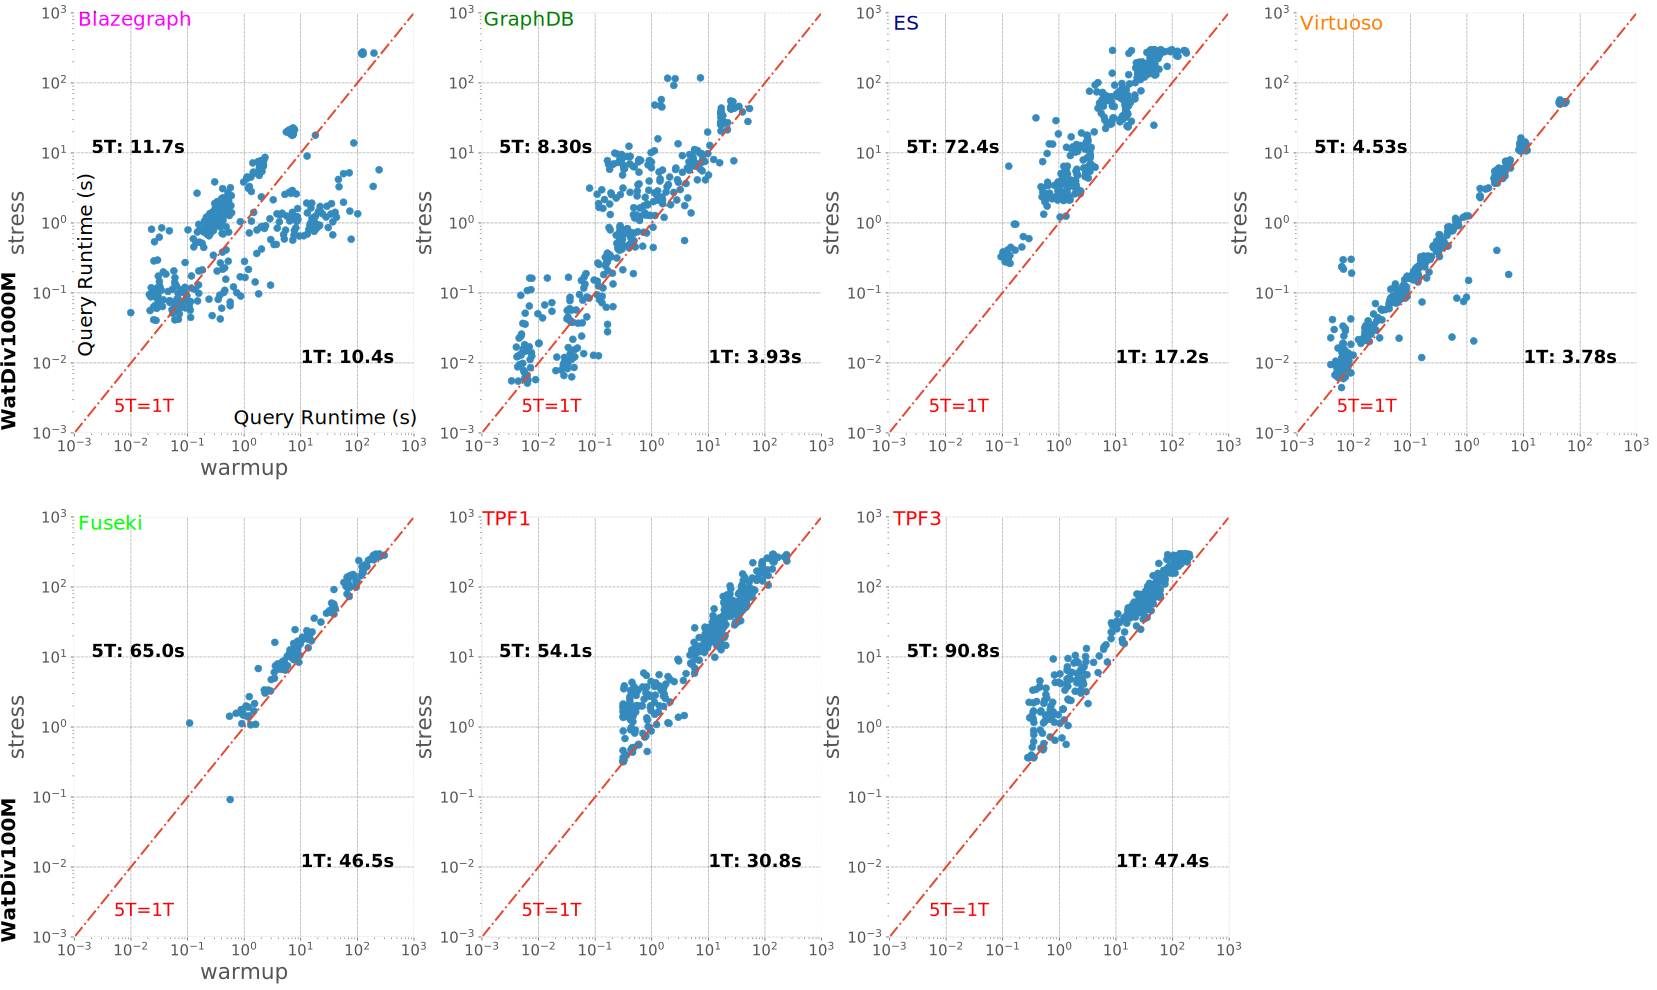
\includegraphics[width=0.90\linewidth]{imgs/Fig07_Watdiv_SingleMultiClient}
	\caption{Runtimes for single versus multi-client workloads: 1 vs. 5 threads. 
		5T runtime corresponds to the maximum runtime per query in the stress test, 1T is the runtime during the warm-up phase. The red line corresponds to the bisector, where the runtime for both workloads is equal. Dots are expected to be shifted up, which correspond to a multiplication factor. The closer the dots to the bisector the smaller the multi-client overhead. Dots below the bisector can be attributed to the natural variance in query runtimes. Average runtimes per store are also shown. \textbf{Bla1\_64} and \textbf{Vir1\_64} have the smallest overhead $(< 20\%)$, for \textbf{ES1\_64} has the largest $(> 300\%)$.
	}
	\label{fig:Fig07_Watdiv_SingleMultiClient}
\end{figure*}
%
%RESULTS Rev1: Notebook Rev1_11 
%results
%1T vs 5T are the runtime of the MEAN query!
%5T runtime corresponds to the max runtime of a query in the stress test, 1T is the runtime during the warmup phase, 5T was chosen max to try and suppress caching effects, therefore fluctuations might be mainly attributed to gaussian noise
%FIGure Caption
%Runtimes for single versus multi-client workloads: 1 vs. 5 threads. 
%5T runtime corresponds to the maximum runtime per query in the stress test, 1T is the runtime during the warmup phase. The red line corresponds to the bisector, where the runtime for both workloads is equal. Dots are expected to be shifted up, which correspond to a multiplication factor. The closer the dots to the bisector the smaller the multi-client overhead. Dots below the bisector can be attributed to the natural variance in query runtimes. Average runtimes per store are also shown. \textbf{Bla1\_64} and \textbf{Vir1\_64} have the smallest overhead $(< 20\%)$, for \textbf{ES1\_64} has the largest $(> 300\%)$.
All results so far focused on the multi-threaded benchmark run, in which 5 benchmark clients are simultaneously executing the same query-mix in a (different) randomized order. It is however interesting to take into account the effect of server load. In Figure~\ref{fig:Fig07_Watdiv_SingleMultiClient} we compare, per query, the runtime of the warm-up run versus the runtime of the slowest multi-threaded run. We chose the slowest query as this has the highest probability of eliminating the effects of caching which will be studied in the next section. Note that for the \emph{SemWeb} systems the comparison is on WatDiv100M, while the \emph{Vendor} systems are compared on WatDiv1000M.

%Bla, Gra, ES, Vir, Fus, TPF1, TPF3
%11.7	10.4		1.125
%8.3	3.93		2.1119592875
%72.4	17.2		4.2093023256
%4.53	3.78		1.1984126984
%65		46.5		1.3978494624
%54.1	30.8		1.7564935065
%90.8	47.4		1.9156118143

\begin{itemize}
	\item \textbf{Highest resilience against server loads}: The lowest multiplication factors (mf) are 1.1 , 1.2, and 1.4 for \textbf{Vir1\_64\_Opt}, \textbf{Bla1\_64\_Opt}, and \textbf{Fus1\_64\_Def} respectively. 
	 
	\item \textbf{Lowest resilience against server loads:} For \textbf{TPF*\_64\_Def} the mf is 1.8 - 1.9.  \textbf{Gra1\_64\_Opt}'s mf is at 2.1, but for \textbf{ES1\_64\_Opt} we have an mf of 4.2.
	
	\item \textbf{Variance of query runtimes:} For Blazegraph and GraphDB the variance on the query runtimes might still be explained as the result of caching. As we will see in the next section however, caching only plays a role for the slow-running queries (\textbf{C}-templates) in the case of Blazegraph.
\end{itemize}


\subsection{The Role of Caching in Query Runtime Results}
\label{subsec:caching}
%
%RESULTS Rev1: Notebook Rev1_08 and Rev1_09 
%TODO study number is notebook 09

%RESULTS ORIGINAL PAPER
%NONE


Some data stores cache the results of queries. Especially in a benchmark where the same query is executed multiple times, this might lead to a large variance on the query runtimes. Although the approach with query events was not designed with support for studying caching effects in mind, having the order of the queries suffices. 
In an initial attempt we plotted the query runtimes as a function of the distance to their nearest preceding execution. For this distance we experimented with the number of intermediary queries, the total number of intermediary results, and the amount of time in between. Results were very similar but did not show any clear pattern. 
In Figure~\ref{fig:Fig08_Watdiv_caching} however, the speedup with respect to the slowest query execution in the multi-client run is plotted as a function of the actual query runtime. This visualization allows an easy distinction between speedups which are caused by noise, mainly for very short query runtimes, and real caching effects. If no caching effects are present the plot should have all its dots on the X and Y-axis.
%Fig. 8. Speedup in query runtime by comparing all query runtimes in the multi-threaded run with the slowest execution in the stress test. With
%no caching all dots are expected on the X and Y-axis, the latter because of the noise on small query runtimes. If we focus on speedups > 2,
%especially ES1 and TPF* seem to have the highest benefit.
\begin{itemize}
	\item \textbf{Stores with clear caching advantage:} The \textbf{TPF} server instances have NGINX~\cite{nginx} cache enabled. The similarity in results with other stores strengthens the idea that Figure~\ref{fig:Fig08_Watdiv_caching} in fact shows caching behavior for 
	\textbf{TPF*\_64}, \textbf{ES1\_64\_Def}, and \\ \textbf{Gra1\_64\_Opt}.
	
	\item \textbf{Caching differences per template type:} For \textbf{ES1\_64\_Def} and \textbf{Gra1\_64\_Opt} the \textbf{F}-templates (blue) dots correspond to the highest speedups. For \textbf{TPF*\_64} query execution is in general slower than for the other systems, therefore \textbf{L} and \textbf{S}-queries, shift to the right and their speedups become more prominent. Small speedups for \textbf{Bla1\_64} and \textbf{Vir1\_64} are mostly limited to the \textbf{C}-template queries.
	\item \textbf{TPF1 vs TPF3:} As a result of the horizontal data partitioning scheme \textbf{S} and \textbf{F}-queries can be resolved locally for \textbf{TPF3\_64} which explain the higher prevalence in the plot.
\end{itemize}








\begin{figure*}[htbp!]
	\centering
	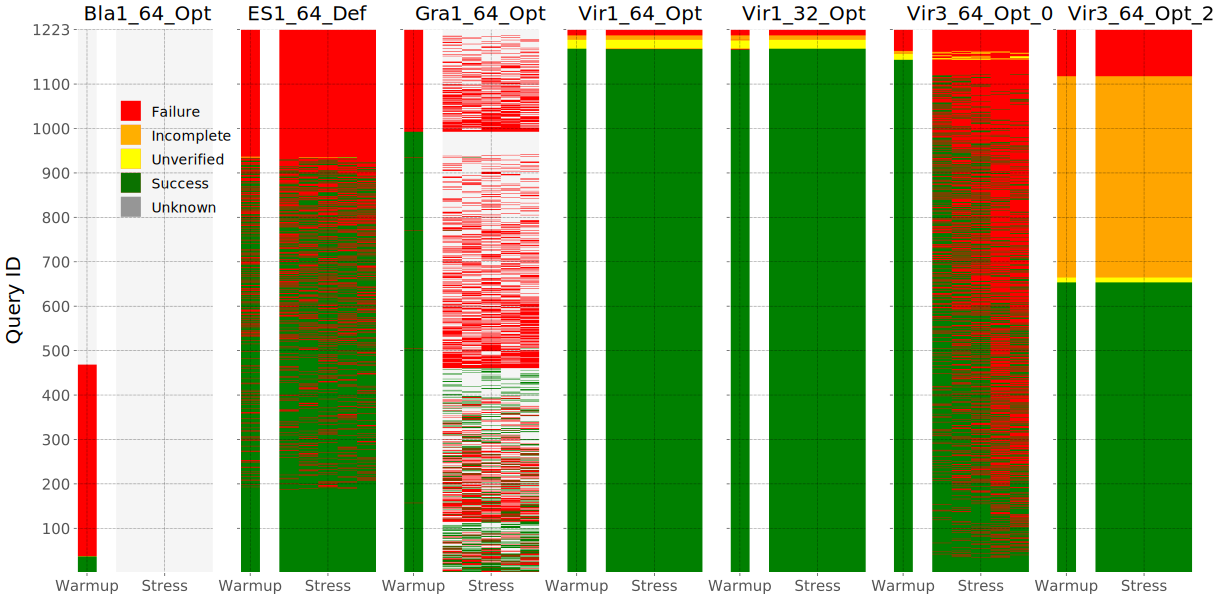
\includegraphics[width=0.90\linewidth]{imgs/Fig09_FailuresOntoforceBM}
	\caption{Overview of successes and errors per query (Y-axis) and thread (X-axis) on the Ontoforce benchmark.
		Queries are sorted per system in order to group error behavior and are not consistent between simulations!
		Blazegraph has a short benchmark survival interval. \textbf{ES1}, \textbf{Gra1} and \textbf{Vir3} Cluster setups have a lot of errors but most queries execute successfully at least once, which allows runtime comparisons. \textbf{Vir3\_64\_Opt\_0} is the most successful Virtuoso cluster run as query completeness analysis revealed that \textbf{Vir3\_64\_Opt\_2} has unreported errors for 37\% of the queries.
	}
	\label{fig:Fig09_FailuresOntoforceBM}
\end{figure*}



\subsection{Query Result Completeness}
\label{subsec:completeness}

In our SWAT4LS contribution~\cite{dewitte_swat4ls_2016} we discovered that query runtimes cannot be trusted without paying careful attention to query completeness. We revisited earlier results on WatDiv and discovered some inconsistencies as well.
\begin{itemize}
	\item \textbf{Vir*\_Def:} Running Virtuoso with the \emph{Default} configurations gave it an advantage since in this setting the result count is limited to $100,000$. This only affects the \textbf{C3} queries for all sizes of WatDiv.
	\item \textbf{Vir*\_Opt:} \textbf{Bla1\_64\_Opt} was the only engine to correctly solve all \textbf{C3} templates. This query returns the highest number of results: 42,063,279. Although Virtuoso was configured to report an unlimited number of results, we discovered that for multiple independent queries the result count is limited to the magic number: 1,048,576. (which is $2^{20}$).  
\end{itemize}
As mentioned in the introduction of section~\ref{sec:tradeoffs} none of the runtime results reported so far are affected by this query incompleteness as we discarded all queries for which at least one store had a different number of results as compared to the consensus. In practice this means that all \textbf{C3} queries had to be discarded. The impact on the runtime comparisons is big as \textbf{C3} has the highest runtimes and ignoring query completeness would put Blazegraph at a serious disadvantage.
